% ***********************************************************
% ******************* PHYSICS HEADER ************************
% ***********************************************************
% Version 2
\documentclass[12pt]{article}
\usepackage{listings}
\usepackage{amsmath} % AMS Math Package
\usepackage{amsthm} % Theorem Formatting
\usepackage{amssymb}    % Math symbols such as \mathbb
\usepackage{graphicx} % Allows for eps images
\usepackage[dvips,letterpaper,margin=1in,bottom=0.7in]{geometry}
\usepackage{tensor}
 % Sets margins and page size
\usepackage{amsmath}
\usepackage{fancyhdr}
\pagestyle{fancy}
\lhead{wc369}
\renewcommand{\labelenumi}{(\alph{enumi})} % Use letters for enumerate
% \DeclareMathOperator{\Sample}{Sample}
\let\vaccent=\v % rename builtin command \v{} to \vaccent{}
\usepackage{enumerate}
\renewcommand{\v}[1]{\ensuremath{\mathbf{#1}}} % for vectors
\newcommand{\gv}[1]{\ensuremath{\mbox{\boldmath$ #1 $}}} 
% for vectors of Greek letters
\newcommand{\uv}[1]{\ensuremath{\mathbf{\hat{#1}}}} % for unit vector
\newcommand{\abs}[1]{\left| #1 \right|} % for absolute value
\newcommand{\avg}[1]{\left< #1 \right>} % for average
\let\underdot=\d % rename builtin command \d{} to \underdot{}
\renewcommand{\d}[2]{\frac{d #1}{d #2}} % for derivatives
\newcommand{\dd}[2]{\frac{d^2 #1}{d #2^2}} % for double derivatives
\newcommand{\pd}[2]{\frac{\partial #1}{\partial #2}} 
% for partial derivatives
\newcommand{\pdd}[2]{\frac{\partial^2 #1}{\partial #2^2}} 
% for double partial derivatives
\newcommand{\pdc}[3]{\left( \frac{\partial #1}{\partial #2}
 \right)_{#3}} % for thermodynamic partial derivatives
\newcommand{\ket}[1]{\left| #1 \right>} % for Dirac bras
\newcommand{\bra}[1]{\left< #1 \right|} % for Dirac kets
\newcommand{\braket}[2]{\left< #1 \vphantom{#2} \right|
 \left. #2 \vphantom{#1} \right>} % for Dirac brackets
\newcommand{\matrixel}[3]{\left< #1 \vphantom{#2#3} \right|
 #2 \left| #3 \vphantom{#1#2} \right>} % for Dirac matrix elements
\newcommand{\grad}[1]{\gv{\nabla} #1} % for gradient
\let\divsymb=\div % rename builtin command \div to \divsymb
\renewcommand{\div}[1]{\gv{\nabla} \cdot \v{#1}} % for divergence
\DeclareMathOperator*{\argmin}{arg\,min}
\newcommand{\curl}[1]{\gv{\nabla} \times \v{#1}} % for curl
\let\baraccent=\= % rename builtin command \= to \baraccent
\renewcommand{\=}[1]{\stackrel{#1}{=}} % for putting numbers above =
\providecommand{\wave}[1]{\v{\tilde{#1}}}
\providecommand{\fr}{\frac}
\providecommand{\RR}{\mathbb{R}}
\providecommand{\NN}{\mathbb{N}}
\providecommand{\seq}{\subseteq}
\usepackage{mathtools}
\DeclarePairedDelimiter{\ceil}{\lceil}{\rceil}
\providecommand{\e}{\epsilon}
\newtheorem{prop}{Proposition}
\newtheorem{thm}{Theorem}[section]
\newtheorem{axiom}{Axiom}[section]
\newtheorem{p}{Problem}[section]
\usepackage{cancel}
\usepackage[font={small,it}]{caption}
\newtheorem*{lem}{Lemma}
\theoremstyle{definition}
\newtheorem*{dfn}{Definition}
 \newenvironment{s}{%\small%
        \begin{trivlist} \item \textbf{Solution}. }{%
            \hspace*{\fill} $\blacksquare$\end{trivlist}}%
\newcommand{\twopartdef}[4]
{
	\left\{
		\begin{array}{ll}
			#1 & \mbox{if } #2 \\
			#3 & \mbox{if } #4
		\end{array}
	\right.
}
\setlength\parindent{0pt}	
% ***********************************************************
% ********************** END HEADER *************************
% ***********************************************************

\begin{document}

{\noindent\Huge\bf  \\[0.5\baselineskip] {\fontfamily{cmr}\selectfont Daily Fantasy Basketball Picker}         }\\[2\baselineskip] % Title
{ {\bf \fontfamily{cmr}\selectfont Automated Decision Systems}\\ {\textit{\fontfamily{cmr}\selectfont     Dec 20 2015}}}~~~~~~~~~~~~~~~~~~~~~~~~~~~~~~~~~~~~~~~~~~~~~~~~~~~~~~~~~~~~~~~~~~~~~~~~~~~~~\
{\large \textsc{ \\William Cai, David Hatch, Evan Green}} % Author name
\\[1.4\baselineskip] 
\section{Introduction} 
\label{in}
 
Daily Fantasy Sports, or DFS, is a new type of sports betting which has recently come into vogue.  Because there is some element of skill, prosecutors have been unable to shut it down in the majority of the country.  In this paper, we will detail an automated decision system that we have constructed, using various paradigms of decision making, to play Daily Fantasy sports.  Section \ref{ps} gives a detailed explanation of the fantasy sports problem along with a mathematical problem statement.  Section \ref{da} breaks down our various data sources and methods for scraping them.  It also explains the database we use to hold the data.  Section \ref{cl} contains our methodology for cleaning the data into the final features we base the model on.  Section \ref{mo} explains how our linear regression algorithm of choice works, and gives a human-friendly explanation of the model. In section \ref{li} we talk about how we generate our lineups using our projections.   In section \ref{ga} we put our money where our mouths are and bet on our lineups.  Finally, in section \ref{in}, we explain how to run the program and what the requirements are. 

\section{Problem Statement} 
\label{ps}
Our goal is to create a program that creates lineups will win the most money on DraftKings as possible. The way we attempt to do this is by creating lineups with the highest expected values and the lowest variance. We use this strategy of high expected values with low variance is because we are designing our algorithm to work best in the "Double Up contests" that DraftKings puts on. In these contests, there is some entry fee and the top 45\% of lineups by points scored double their entry fee. The expected value of these contests is just 90\% of the contest fee assuming that we enter an average lineup. However, by creating lineups with with the highest expected points, we can hopefully raise our expected value over the break even point of the entry fee. Low variance is best for this type of contest because very high values are not better than just moderately high values. High expected value is also good for this type of contest because the top 45\% of lineups by points. 

\section{Getting the Data} 
\label{da}
\emph{The code referenced in this section is located in bin/scrape, bin/load\_db, schneiderman/scrape, and schneiderman/models}\\

To gather the data, we downloaded game logs for every current NBA player using the NBA.com API. Scraping the NBA API leads to JSON files which are then combed for the relevant information. This data was then fed into a database that had three types of data models. The first of these is a Player class. Objects in the player class have a unique id, which is used to index the database. They also contain information about the player's name on NBA.com and DraftKings.com so that we can access information on either site, the player's team, and the set of games that the player has played in this season. One of the other classes in the database is the Team class. The team class contains fields for the team's name, NBA.com abbreviation, and the DraftKings abbreviation to enable looking up the team on both websites. It also contains information about the team's relative strength. The PlayerGame class includes the information about a specific players stats on a specific game. These are the statistics that are used by DraftKings to calculate daily fantasy scores. The PlayerGame also includes fields for that player's database entry and the opponents database entry. These fields are very important for the cleaning step. 

\section{Cleaning the Data} 
\label{cl}
\emph{The code referenced in this section is located in bin/clean}\\

After we have scraped the data into the database, we produce game log files that can be used to run the regression. The output of this step is multiple csv files that on each line contains a single player game. The row is made up of the predictor variables and the daily fantasy points that the player scored on that day. Some of the predictor variables are running averages for previous 1, 5 and 10 games of all the statistics that are used to calculate daily fantasy points. We also added categorical variables for the opponent because who the player is playing can have large effects on the statistics of the player in that game. Additional predictor variables are if the game is home or not and the number of days since the last game. All of the regression models are run on individual positions so this step also separates the players into their respective positions. It is split up into the respective positions because DraftKings requires that lineups generated have a specific number of each position. Therefore, players are compared more to their own positions than to players of other positions. Finally, this step deletes all the games for which players did not appear because it wouldn't make sense to try to predict the players scores in those games. 


\section{Learning the models} 
\label{mo}
\emph{The code related to this section is in the regression folder in the schneiderman/regression/predict.py and schneiderman/regression/regress.py files } \\

Our linear regression algorithm of choice was the elastic net, a form of regularized linear regression.  It was important to choose from the family of regularized linear regression because we have a pretty small ratio of data points to features, and we wanted the ability to add as many features as we wanted.  Doing linear regression on a dataset with comparable amounts of features to data points quickly becomes an exercise in creating ridiculous models because of the danger of overfitting.  Regularization combats this trend by adding in a term based on the coefficients of the model to the loss function of linear regression, which is simply the residual sum of squares.  \\

There are several regression methods in the regularized linear regression family.  The most popular of these are the LASSO, ridge regression, and elastic net.  Our choice, elastic net, is an interpolation between the other two and has several properties which lend themselves to our project.  For one, given a group of correlated variables, of which we have many, the elastic net will give all of them a coefficient.  This is in contrast to the LASSO, which will arbitrarily select one and give it a coefficient and set the rest to 0.  Using the elastic net allows us to better understand our program's explanation of it's decisions.  The advantage that the elastic net has over ridge regression is that it will zero out some variables, which will allow us to say which of our features give no signal - another useful way for us to understand which features are important in predicting fantasy scores.  On the other hand, ridge regression will almost never set a coefficient to zero, making interpretation more difficult.  
\begin{figure}
$$\beta_{elastic net}  = \argmin\limits_\beta (||y - X \beta ||^2 + \lambda_2||\beta||^2 + \lambda_1||\beta||_1)$$
$$\beta_{LASSO}  = \argmin\limits_\beta (\frac{1}{N}||y - X \beta ||_2^2 + \lambda||\beta||_1)$$
$$\beta_{ridge}  = \argmin\limits_\beta (||y - X \beta ||^2 + \lambda||\beta||^2 )$$
\caption{The cost functions of various regression methods in the regularized linear regression family.  Note how elastic net contains the terms from both the LASSO and ridge regression.}

\end{figure}\\


In our code, we read in each player-game for each position from a csv file which was produced from our data cleaning.  Each line of the csv is of form\\
$x_1, x_2, ..., x_n, y, $player-name
We then load that into numpy matrices X and Y, where X is $num_{player-games} $by n and Y is $num_{player-games}$ by 1, and use numpy's elastic net, ElasticNetCV, to find a linear model $\beta$ which solves 
$$\beta  = \argmin\limits_\beta (||y - X \beta ||^2 + \lambda_2||\beta||^2 + \lambda_1||\beta||_1)$$

The $\lambda$s are learned through three-fold cross validation, which splits the data into thirds and learns it on two thirds at a time, using the last third for validation.  The elastic nets are made for a variety of $\lambda$s, and the $\lambda$s which have the lowest error are used.  Furthermore, note that all features are regularized before using the elastic net to allow for the coefficients to be penalized equally.  Mathematically, this means that for each feature $x_i$ we subtract the mean of the $x_i$ such that $$\sum\limits_{j=1}^n x_j(i) = 0$$ Where $x_j(i)$ denotes the ith feature of the jth player-game.  We then divide each $x_j(i)$ by the standard deviation of the $x_i$s.  

The result of this is a linear model for each position, which predicts how many daily fantasy points.  The models, along with an interpretation, are given in files models.pdf.  They are not included here because there are over 100 features so it would take the majority of the paper.  

Given these models, we can generate the expected value of fantasy points for each player by plugging their scraped data into the model.  We can further generate their variance by going through their projections for previous games and seeing how much they deviate from the model.  This allows us to generate our expectedvalues and residPOSITION csv files.  Each row of expectedvalues is of form \\

Name, position, expected daily fantasy points, salary\\

and each row of residPOSITION is of form \\

Name, standard deviation \\

Our lineup generator will read in these files and use them to generate lineups with high expected value and low variance.

\section{Generating the lineups} 
\label{li}
\emph{The code referenced in this section is found in the lineup folder, in bin/set\_lineups.py } \\

Now that we have the projections, we need to generate some lineups to submit that we hope will make money!  A formalization of this problem is as follows: \\

Given a list P of players, we would like to generate a set of lineups L s.t. given a lineup $L_i$ in L, the sum of the expected values of the players of $L_i$ is close to maximized under the constraint that the the sum of the salaries of the players of $L_i$ do not exceed a maximum salary.  \\
 
Any computer scientist will see this as a variation of the weighted knapsack problem, which is a classic NP-hard problem.  However, our problem has several constraints which make it easier to solve, along with some other twists.\\

1)We are only interested in solving this problem for a budget of \$50,000, because that's what every contest on DraftKings(a popular DFS website) uses.  \\
2)Player salaries are all contained within the range from \$3000 to \$11000.  \\
3)Players have variances along with their expected scores (we are using a gaussian model).  Because we are specifically interested in double-up games, our ideal lineup is one which is high expected value and low variance, because it maximizes the chance of getting into the money.  \\
4)Because players can be used across many lineups, we must make sure that our set of lineups L does not depend too heavily on the performance of a small number of players.  Otherwise, if those players had a bad game our bankroll would be entirely wiped out.  \\
5)It's not entirely clear what the threshold for finishing in the money is - this varies quite a bit between days depending on how many players which are used in other people's lineups have good days.  \\

The algorithm we came up with has three separate stages which address these issues.

\subsection{Thresholding}
The code that does the process described in this subsection is located at the beginning of the main() submodule in set\_lineup.py. 

Before we begin generating lineups, we need to figure out our threshold for expected value for the lineups (we will reject lineups whose expected value is below this).  We decide to do this by generating lineups using our lineup generator (discussed in the next section, section \ref{ge}) and taking the minimum expected value of lineups in the top X\%.  \\

X was tuned using past data by selecting an X such that on average, our threshold was above the money.  Note that we can't just lower X to arbitrarily low numbers, because then we may be unable to find lineups and they will heavily depend on the same players.  Furthermore, by getting some breathing room with a slightly higher X, we are able to focus more on variance, increasing the chances that our lineups make money. We set X=2.  We will call this threshold T.  \\

\subsection{Lineup Generator}
\label{ge}
The code described in this subsection is in the get\_lineup() submodule in set\_lineup.py 

Given this threshold T, we want to write a submodule which can generate a single lineup with an expected value above T but with a budget under our salary cap.  We use a greedy randomized algorithm:\\

1)Randomize the order of the positions to be picked out of PG, SG, SF, PF, C, G, F, UTIL.  This will allow us to get a healthy selection of players.  \\
2)For each position, randomly select a player, where each player has $\frac{expected value}{salary}$ chance of being chosen, making sure we have enough money left to fill out our roster.  Then adjust the remaining salary.\\
3)After having chosen a player for each position, we will have some amount of money left over.  Re-randomize the positions.\\
4)For each position, pick a random player according to the same probability distribution.  If that player has higher expected value and fits our salary constraints, replace the current player for that position with him and adjust the salary accordingly.  \\
5)Repeat steps 3-4 until there are no more possible improvements.\\

Through experimentation, we found that this typically generates a lineup that uses almost all of the salary and has close to maximum expected-value/salary ratio, meaning that we have succeeded in generating lineups with expected value above T. Note that this algorithm works well because of the small range in salaries (constraints 1 and 2 in our list).  

\subsection{List of Lineups generator}
\label{lge}
\emph{The code which contains the algorithm described in this section is in the main() submodule in set\_lineup.py} \\

Now that we have a tool for generating a single lineup, we would like to be able to generate a list of lineups. However, as mentioned in our list of constraints, we want to make sure the list is not too dependent on certain players.  We invented a novel algorithm to solve this problem, which we call the box algorithm (it is a flavor of Monte Carlo):\\

1) Fill a box with n lineups, where n is the number of lineups you would like to generate.  \\
2) Shake the box k times, where a box shake is defined as follows: \\
a) For each player, assign the player a score by sampling a number from a normal distribution centered at his expected value with standard deviation equal to his past standard deviation.  \\
b) For each lineup in the box, add the scores of the players. Compute the median score. \\
c) For each lineup in the box below the median score, flip a coin.  If it's heads, remove the lineup from the box.   \\
d) For each lineup that was removed from the box, add a new lineup from get\_lineup into the box. \\
\\

After k shakes, we print all the lineups in the box.  We order these in the number of shakes that the lineup has survived, with the lineups surviving the most shakes (which we expect to be the best lineups) at the top.  k is set to be an arbitrarily large number, typically on the order of the size of the box.  \\

The rationale behind the box shaking is that if a single player has a bad game, many of the lineups depending on it will be removed from the box, which will remove dependencies on certain players.  

\section{Taking it out for a spin!}
\label{ga}
We will use our model to predict the games on Monday December 21.   You can see a visual representation of our linear regression model in our appendix. In the appendix, the features whose points are farthest away from the x-axis are the most significant.  The features that we found to be most significant for each of the 5 NBA positions are: \\

C: Minutes Played - last 10 games, Minutes Played - last 5 game, Points -  last 10 games, Opp-Chi, Opp-NY, Opp-UTA, DefensiveRebounds-10 \\

PF: Minutes Played -  last 10 games, Minutes Played - last 5 games, Opp-PHO, Field Goal Attempts - last 10 games, Turnovers - last 10 games, Steals - last 10 games, Points - last 10 games \\

SF:��Minutes Played -  last 10 games, Minutes Played - last 5 games, Opp-Hou, Opp-Cle, Points- last 10 games, FieldGoalAttempts - last 10 games, defensive rebounds - last 10 games\\

SG: Minutes Played -  last 10 games, Minutes Played - last 5 games, Opp-Was, FieldGoalAttempts - last 10 games, defensive rebounds - last 10 games, points - last 10 games \\

PG: Minutes Played -  last 10 games, Minutes Played - last 5 games, FieldGoalAttempts - last 10 games, defensive rebounds - last 10 games, points - last 10 games, steals- last 10 games,FieldGoalAttempts - last 5 games \\

In figure 2, we show off the UI of our program, which is on the command line. \\

You can see the generated lineups in figure 3.  
\begin{figure}[h]
\label{lines}
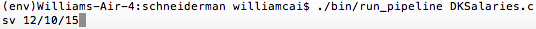
\includegraphics{ui.png}
\caption{A screenshot of how to run our program}
\end{figure}


\begin{figure}
\label{lines}
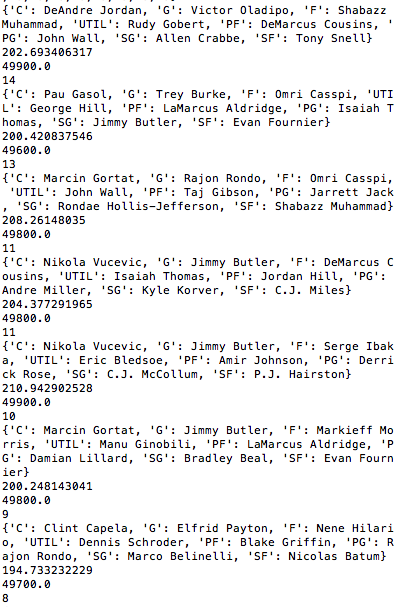
\includegraphics{lineups.png}
\caption{A screenshot of the lineups it generated, followed by their expected points scored, total salary cost of the team, and number of shakes of the box it survived}
\end{figure}
\newpage


\section{Installing depended packages}
\label{in}
First, clone the github repository by running  \\

git clone https://github.com/dhatch/schneiderman.git \\

Change into the project directory by running \\

cd schneiderman \\

First, you should create a virtual environment with the command\\

virtualenv env \\

Then activate the environment with the command \\

source env/bin/activate\\

Then, to install the depended packages, use the command \\

pip install -r requirements.txt  \\

The packages required are lxml, numpy, pandas, requests, scipy, iphython, python-dateutil, pony, docopt, fuzzywuzzy, python-Levenshtein, and scikit-learn. \\

Then, \\

source ./bin/set\_env \\

To run the program use the command \\

./bin/run\_pipeline DKSalaries.csv 12/21/15

which will run all the requisite files in order. \\

./bin/run\_pipeline takes two parameters. The first parameter is the csv file downloaded from Draftkings.com. There is one in the samples folder labeled as "DKSalaries.csv". The second parameter is the date of the contest, which for the sample is 12/21/15. Running this prints our recommended lineups, expected points, and salary to stdout. 

 \end{document}